\chapter{Strutture dati}
\section{Introduzione}
Iniziamo con delle definizioni:
\begin{definition}[Dato]
    In un linguaggio di programmazione, un dato è un valore che una variabile
    può assumere.
\end{definition}
\begin{definition}[Tipo di dato astratto]
    Un tipo di dato astratto è un modello matematica dato da una collezione di
    valori e un insieme di operazioni ammesse su questi valori.
\end{definition}
\begin{definition}[Tipo di dato primitivo]
    Un tipo di dato fornito direttamente da un linguaggio è detto essere
    primitivo.
\end{definition}
\begin{definition}[Specifica e implementazione di un tipo di dato]
    Per ogni tipo di dato astratto si definiscono due livelli:
    \begin{itemize}
        \item \emph{Specifica}: costituisce l'interfaccia di utilizzo del tipo
        di dato e ne nasconde i dettagli implementativi;
        \item \emph{Implementazione}: è la realizzazione vera e propria del tipo
        di dato;
    \end{itemize}
\end{definition}\noindent
I seguenti sono esempi di \emph{specifica} e \emph{implementazione} di un
\emph{tipo di dato}:
\begin{table}[h]
    \centering
    \renewcommand{\arraystretch}{1.2}
    \begin{tabular}{|c|c|}
        \hline
        \textbf{Specifica} & \textbf{Implementazione}\\
        \hline
        Numeri reali & IEEE754\\
        \hline
        Pile & \parbox[t]{6cm}{Pile basate su vettori\\
        Pile basate su puntatori}\\
        \hline
        Code & \parbox[t]{6cm}{Code basate su vettori circolari\\
        Code basate su puntatori}\\
        \hline
    \end{tabular}
\end{table}

\begin{definition}[Struttura di dati]
    Una struttura di dati è una collezione di dati caratterizzata dalla struttura
    della collezione, piuttosto che dal tipo dei dati contenuti.
\end{definition}\noindent
Una \emph{struttura di dati} è caratterizzata da un insieme di operatori che
consentono di manipolarne la struttura e da un modo sistematico di organizzare i
dati in essa contenuti.

Le \emph{strutture di dati} possono essere categorizzate sulla base di tre
parametri:
\begin{itemize}
    \item \emph{Lineari/Non lineari}: se è presente o meno una sequenza;
    \item \emph{Dinamiche/Statiche}: se è possibile modificare o meno la dimensione
    della struttura dopo averla creata;
    \item \emph{Omogenee/Disomogenee}: se i dati contenuti sono tutti dello stesso
    tipo o di tipi diversi;
\end{itemize}

\section{Strutture di dati astratte}
\subsection{Sequenze}
\begin{definition}[Sequenza]
    Una sequenza è una struttura dati dinamica e lineare rappresentante una
    sequenza ordinata di valori che possono comparire anche più di una volta.
\end{definition}
\begin{note}
    L'ordine dei valori all'interno di una \emph{sequenza} è importante!
\end{note}

\paragraph{Operazioni ammesse}
Su una \emph{sequenza} sono ammesse le seguenti operazioni:
\begin{itemize}
    \item Data una posizione è possibile aggiungere o togliere elementi, cioè
    se $s=s_1,\,s_2,\,\dots,\,s_n$ è la \emph{sequenza}, l'elemento $s_i$ è in
    posizione $pos_i$, inoltre, esistono posizioni fittizie quali $pos_0$ e
    $pos_{n+1}$ che rappresentano la posizione del primo elemento e dell'elemento
    successivo a quello in $pos_n$;
    \item Accesso diretto alla testa o alla coda;
    \item Accesso sequenziale alle altre posizioni;
\end{itemize}

\paragraph{Specifica}
\begin{code}{Sequenza}
\com{Restituisce \bc{true} se la sequenza è vuota}
\bc{boolean} isEmpty()
\nl\com{Restituisce \bc{true} se $p=pos_0$ o se $p=pos_{n+1}$}
\bc{boolean} finished(\bc{POS} p)
\nl\com{Restituisce la posizione del primo elemento}
\bc{POS} head()
\nl\com{Restituisce la posizione dell'ultimo elemento}
\bc{POS} tail()
\nl\com{Restituisce la posizione dell'elemento che segue $p$}
\bc{POS} next(\bc{POS} p)
\nl\com{Restituisce la posizione dell'elemento che precede $p$}
\bc{POS} prev(\bc{POS} p)
\nl\com{Inserisce l'elemento $v$ di tipo \bc{ITEM} nella posizione $p$ e
restituisce}
\com{la posizione del nuovo elemento, che diviene il predecessore di $p$}
\bc{POS} insert(\bc{POS} p, \bc{ITEM} v)
\nl\com{Rimuove l'elemento contenuto nella posizione $p$ e restituisce la
posizione}
\com{del successore di $p$, che diviene il successore del predecessore di $p$}
\bc{POS} remove(\bc{POS} p)
\nl\com{Legge l'elemento di tipo \bc{ITEM} contenuto nella posizione $p$}
\bc{ITEM} read(\bc{POS} p)
\nl\com{Scrive l'elemento $v$ di tipo \bc{ITEM} nella posizione $p$}
write(\bc{POS} p, \bc{ITEM} v)
\end{code}

\subsection{Insiemi}
\begin{definition}[Insieme]
    Un insieme è una struttura dati dinamica e non lineare che memorizza una
    collezione non ordinata di valori non ripetuti.
\end{definition}
\begin{note}
    L'ordinamento fra elementi è dato dall'eventuale relazione d'ordine
    definita sul tipo degli elementi stessi.
\end{note}

\paragraph{Operazioni ammesse}
Su un \emph{insieme} sono ammessi diversi tipi di operazioni:
\begin{itemize}
    \item \emph{Operazioni di base}:
    \begin{itemize}
        \item Inserimento;
        \item Rimozione;
        \item Test di appartenenza;
    \end{itemize}
    \item \emph{Operazioni di ordinamento}: estrazione valore massimo/minimo;
    \item \emph{Operazioni insiemistiche}:
        \begin{itemize}
            \item Unione;
            \item Intersezione;
            \item Differenza;
        \end{itemize}
    \item \emph{Iterazione sugli elementi}: esecuzione di operazioni su tutti
    gli elementi dell'\emph{insieme} (e.g. \texttt{foreach (x $\in$ S) do \dots});
\end{itemize}

\paragraph{Specifica}
\begin{code}{Insieme}
    \com{Restituisce la cardinalità dell'\emph{insieme}}
    \bc{int} size()
    \nl\com{Restituisce \bc{true} se $x$ è contenuto nell'\emph{insieme}}
    \bc{boolean} contains(\bc{ITEM} x)
    \nl\com{Inserisce $x$ nell'\emph{insieme}, se non è giù presente}
    insert(\bc{ITEM} x)
    \nl\com{Rimuove $x$ dall'\emph{insieme}, se è presente}
    remove(\bc{ITEM} x)
    \nl\com{Restituisce un nuovo \emph{insieme} che è l'unione di $A$ e $B$}
    \bc{Set} union(\bc{Set} A, \bc{Set} B)
    \nl\com{Restituisce un nuovo \emph{insieme} che è l'intersezione di $A$ e $B$}
    \bc{Set} intersection(\bc{Set} A, \bc{Set} B)
    \nl\com{Restituisce un nuovo insieme che è la differenza di $A$ e $B$}
    \bc{Set} difference(\bc{Set} A, \bc{Set} B)
\end{code}

\subsection{Dizionari}
\begin{definition}[Dizionario]
    Un dizionario è una struttura dati dinamica che rappresenta il concetto
    matematico di relazione univoca, o associazione chiave-valore, $R:D\to C$,
    dove $D$ è un l'insieme dominio i cui elementi sono detti chiavi e $C$ è un
    insieme codominio di elementi detti valori.
\end{definition}

\paragraph{Operazioni ammesse}
Su un \emph{dizionario} sono ammesse le seguenti operazioni:
\begin{itemize}
    \item Data una chiave è possibile accedere al valore associato o a
    \texttt{nil} se la chiave non è associata a nulla;
    \item Creazione di una nuova associazione chiave-valore, eventualmente
    sostituendo il precedente valore associato a quella chiave;
    \item Eliminazione di un'associazione chiave-valore;
\end{itemize}

\paragraph{Specifica}
\begin{code}{Dizionario}
\com{Restituisce il valore associato alla chiave $k$ se presente, nil altrimenti}
\bc{ITEM} lookup(\bc{ITEM} k)
\nl\com{Associa il valore $v$ alla chiave $k$}
insert(\bc{ITEM} k, \bc{ITEM} v)
\nl\com{Rimuove l'associazione della chiave $k$}
remove(\bc{ITEM} k)
\end{code}

\subsection{Grafi e alberi}
\begin{definition}[Grafo]
    Un grafo è una struttura composta da un insieme di elementi detti nodi o
    vertici e un insieme di coppie di nodi, ordinate o meno, dette archi.
\end{definition}
\begin{definition}[Albero ordinato]
    Un albero ordinato è una struttura dati dinamica composta da un insieme
    finito di elementi detti nodi. Uno di questi nodi è detto radice, tutti gli
    altri sono partizionati in insiemi ordinati e disgiunti che sono anch'essi
    alberi ordinati.
\end{definition}

\begin{figure}[h]
    \centering
    \subfloat[\emph{Grafo} con archi orientati]{
        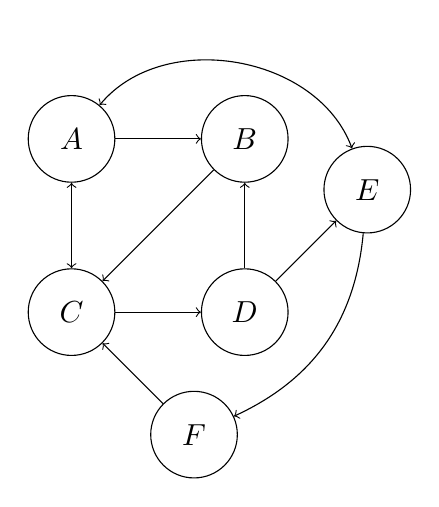
\begin{tikzpicture}[node distance={20mm},main/.style={draw, circle, scale=1.1, minimum size=10mm}]
            \node[main] (0) {$A$};          
            \node[main] (1) [right of=0] {$B$};
            \node[main] (2) [below of=0] {$C$};
            \node[main] (3) [below of=1] {$D$};
            \node[main] (4) [above right of=3] {$E$};
            \node[main] (5) [below right of=2] {$F$};
          
            \draw[->] (0) -- (1);
            \draw[<->] (0) -- (2);
            \draw[<-] (1) -- (3);
            \draw[->] (2) -- (3);
            \draw[<-] (2) -- (1);
            \draw[->] (3) -- (4);
            \draw[<-] (2) -- (5);
            \draw[<->] (0) edge[bend left=60] (4);
            \draw[<-] (5) edge[bend right] (4);
          \end{tikzpicture}
    }
    \hspace{1.5cm}
    \subfloat[\emph{Albero ordinato}]{
        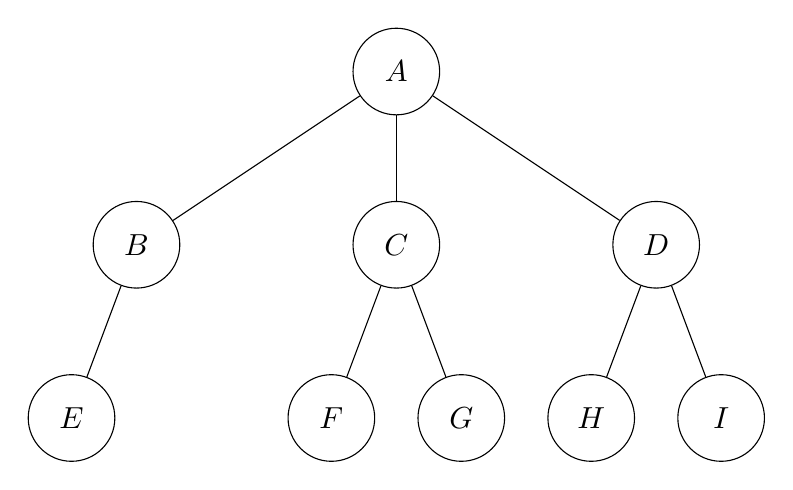
\begin{tikzpicture}[node distance={20mm},main/.style={draw, circle, scale=1.1, minimum size=10mm}]
            \node[main] (0) {$A$};
          
            \node[main] (2) [below of=0] {$C$};
            \node[main] (1) [left of=2, xshift=-10mm] {$B$};
            \node[main] (3) [right of=2, xshift=10mm] {$D$};
          
            \node[main] (4) [below of=1, xshift=-7.5mm] {$E$};
            \node[main] (5) [below of=2, xshift=-7.5mm] {$F$};
            \node[main] (6) [below of=2, xshift=7.5mm] {$G$};
            \node[main] (7) [below of=3, xshift=-7.5mm] {$H$};
            \node[main] (8) [below of=3, xshift=7.5mm] {$I$};
          
            \path[-]  (0) edge (1)
                      (0) edge (2)
                      (0) edge (3)
                      (1) edge (4)
                      (2) edge (5)
                      (2) edge (6)
                      (3) edge (7)
                      (3) edge (8);
          \end{tikzpicture}
    }
    \caption{\emph{Grafo} VS \emph{Albero ordinato}}
\end{figure}

\paragraph{Operazioni ammesse} Oltre a inserimento e rimozione, le operazioni
ammesse su \emph{grafi} e \emph{alberi} ruotano attorno alla possibilità di
accedere a tutti gli elementi delle strutture secondo diverse
\emph{visite}\footnote{Tutte le \emph{visite} saranno discusse nel dettaglio
nel prossimo capitolo}.

\subsection{Criticità nell'implementazione di strutture dati astratte}
Quando si implementa una \emph{struttura di dati astratta} può essere naturale
prediligere una particolare \emph{struttura di dati elementare} piuttosto che
un'altra. Ad esempio, viene naturale implementare una \emph{sequenza}
usando una \emph{lista}, o un \emph{albero astratto} come \emph{albero di
puntatori}. Tuttavia, esistono possibilità meno scontate, come l'utilizzo di
un vettore di booleani per l'implementazione di un \emph{insieme}, o un
\emph{albero} implementato come \emph{vettore dei padri}.

La \emph{struttura di dati elementare} scelta per l'implementazione di una
\emph{struttura dati astratta} si ripercuote sull'efficienza delle singole
operazioni. Per esempio, un \emph{dizionario} implementato come \emph{tabella
hash} permette di avere \emph{complessità} $O(1)$ nella funzione \texttt{lookup}
e $O(n)$ nella ricerca del minimo. Invece, lo stesso \emph{dizionario}
implementato come \emph{albero} porta la \emph{complessità} della \texttt{lookup}
a $O(\log n)$, ma riduce a $O(1)$ quella per la ricerca del minimo.

\newpage
\section{Strutture di dati elementari}
Vediamo ora le possibili implementazioni delle più comuni \emph{strutture
dati elementari}: \emph{liste}, \emph{pile} e \emph{code}.

\subsection{Liste}
\begin{definition}[Lista]
    Una lista è una sequenza di nodi contenenti dati arbitrati e uno o due
    puntatori all'elemento successivo e/o precedente.
\end{definition}
\begin{note}
    È importante notare che nodi contigui nella \emph{lista} non lo sono
    necessariamente anche in memoria.
\end{note}
\begin{note}
    In una \emph{lista} tutte le operazioni hanno costo $O(1)$.
\end{note}\noindent
Diverse implementazioni di una \emph{lista} possono essere categorizzate sulla
base di tre parametri:
\begin{itemize}
    \item \emph{Monodirezionali/Bidirezionali}: sono \emph{bidirezionali} le
    implementazioni in cui ogni nodo contiene due puntatori: uno all'elemento
    precedente, l'altro al successivo;
    \item \emph{Con sentinelle/Senza sentinella}: sono \emph{con sentinella}
    tutte le implementazioni in cui una \emph{lista} vuota ha un elemento;
    \item \emph{Circolare/Non circolare}: sono \emph{circolari} le
    implementazioni in cui l'ultimo elemento ha come successivo il primo, o
    viceversa;
\end{itemize}

\begin{figure}[ht]
    \centering
    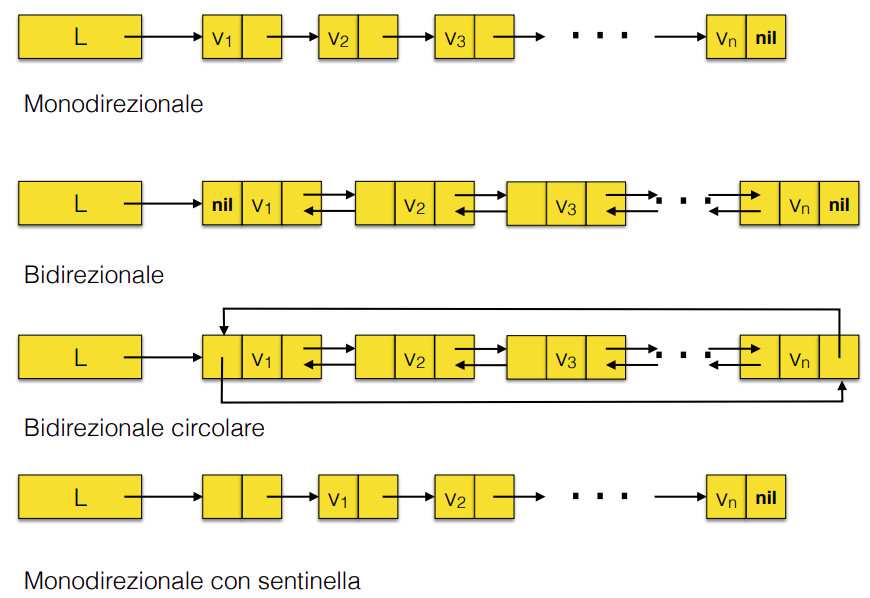
\includegraphics[width=0.9\textwidth]{tipi-liste.png}
    \caption{Diverse implementazioni di una \emph{lista}}
\end{figure}

\paragraph{Implementazione del tipo di dato POS}
\begin{code}{POS}
    \bc{POS} succ\hfill\com{Elemento successivo}
    \bc{POS} pred\hfill\com{Elemento precedente}
    \bc{ITEM} value\hfill\com{Valore}
    
    \ind\bc{POS} Pos(\bc{ITEM} v)\\
        \bc{POS} p = new \bc{POS}\\
        p.succ = nil\\
        p.pred = nil\\
        p.value = v\\
        return p
\end{code}

\paragraph{Implementazione di una lista bidirezionale con sentinella}
\begin{code}{Lista bidirezionale con sentinella}
    \begin{minipage}[t]{0.48\textwidth}
        \bc{LIST} pred\hfill\com{Predecessore}
        \bc{LIST} succ\hfill\com{Successore}
        \bc{ITEM} value\hfill\com{Valore}

        \ind\bc{LIST} List()\\
            \bc{LIST} t = new LIST\\
            t.pred = t\\
            t.succ = t\\
            return t\\

        \ind\bc{boolean} isEmpty()\\
            return (pred == succ == this)\\

        \ind\bc{POS} head()\\
            return succ\\

        \ind\bc{POS} tail()\\
            return pred\\

        \ind\bc{POS} next(\bc{POS} p)\\
            return p.succ\\

        \ind\bc{POS} prev(\bc{POS} p)\\
            return p.pred\\
    \end{minipage}
    \hfill
    \begin{minipage}[t]{0.48\textwidth}
        \par\noindent\com{Restituisce \bc{true} se $p$ è la}
        \com{posizione \emph{sentinella}}
        \rmbreak\ind\bc{boolean} finished(\bc{POS} p)\\
            return (p == this)\\

        \ind\bc{ITEM} read(\bc{POS} p)\\
            return p.value\\

        \ind write(\bc{POS} p, \bc{ITEM} v)\\
            p.value = v\\

        \ind\bc{POS} insert(\bc{POS} p, \bc{ITEM} v)\\
            \bc{POS} t = Pos(v)\\
            t.pred = p.pred\\
            p.pred.succ = t\\
            t.succ = p\\
            p.pred = t\\
            return t\\

        \ind\bc{POS} remove(\bc{POS} p)\\
            p.pred.succ = p.succ\\
            p.succ.pred = p.pred\\
            \bc{POS} t = p.succ\\
            delete p\\
            return t
        
    \end{minipage}
\end{code}
\begin{note}
    I tipi \texttt{POS} e \texttt{LIST} sono equivalenti.
\end{note}
\begin{note}
    Alla posizione \emph{sentinella} non è stato assegnato alcun valore
    in quanto serve soltanto a semplificare le operazioni di inserimento e
    rimozione.
\end{note}

\newpage
\subsection{Pile}
\begin{definition}[Pila]
    Una pila è una struttura dati dinamica e lineare, nella quale l'accesso agli
    elementi è definito in base all'ordine in cui sono stati inseriti. In
    particolare, è possibile accedere direttamente soltanto all'ultimo elemento
    inserito.
\end{definition}
\begin{note}
    Le \emph{pile} sono basate sull'approccio \emph{LIFO} (\emph{Last In, First
    Out}).
\end{note}

\paragraph{Specifica}
\begin{code}{Pila}
    \com{Restituisce \bc{true} se la \emph{pila} è vuota}
    \bc{boolean} isEmpty()
    \nl\com{Inserisce $v$ in cima alla pila}
    push(\bc{ITEM} v)
    \nl\com{Rimuove l'elemento in cima alla \emph{pila} e lo restituisce}
    \bc{ITEM} pop()
    \nl\com{Legge l'elemento in cima alla \emph{pila}}
    \bc{ITEM} top()
\end{code}
\begin{note}
    Nel gergo delle \emph{pile}, l'elemento \q{in cima} è l'ultimo elemento
    inserito, mentre quello \q{in fondo}, il primo.
\end{note}\noindent
Una \emph{pila} può essere implementata come \emph{vettore}, quindi di dimensione
limitata, o come \emph{lista bidirezionale} con puntatore all'elemento in testa.
\begin{figure}[h]
    \centering
    \subfloat[\emph{Pila} implementata come \emph{lista}]{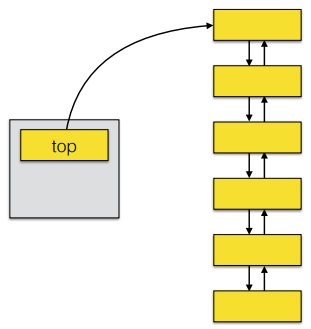
\includegraphics[width=0.4\textwidth, align=c]{pila-lista.png}}
    \hspace*{2cm}
    \subfloat[\emph{Pila} implementata come \emph{vettore}]{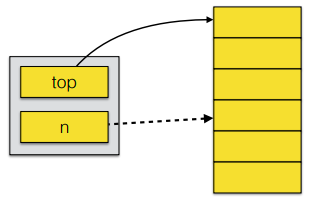
\includegraphics[width=0.4\textwidth, align=c]{pila-vettore.png}}
    \caption{Diverse implementazioni di una \emph{pila}}
\end{figure}

\newpage
\paragraph{Implementazione di una pila basata su vettore}
\begin{code}{Pila basata su vettore}
    \begin{minipage}[t]{0.48\textwidth}
        \bc{ITEM}[] V\hfill\com{Elementi}
        \bc{int} cur\hfill\com{Posizione cursore}
        \bc{int} max\_dim\hfill\com{Dimensione massima}

        \ind\bc{STACK} Stack(\bc{int} dim)\\
            \bc{STACK} t = new \bc{STACK}\\
            t.V = new \bc{int}[1\dots dim]\\
            t.V = new \bc{int}[1\dots dim]\\
            t.cur = 0\\
            t.max\_dim = dim\\
            return t\\
        
        \ind\bc{ITEM} top()\\
            precondition:(cur > 0)\\
            return V[cur]
    \end{minipage}
    \hfill
    \begin{minipage}[t]{0.48\textwidth}
        \ind\bc{boolean} isEmpty()\\
            return (cur == 0)\\

        \ind\bc{ITEM} pop()\\
            precondition:(cur > 0)\\
            \bc{ITEM} t = V[cur]\\
            cur = cur - 1\\
            return t\\

        \ind push(\bc{ITEM} v)\\
            precondition:(cur < max\_dim)\\
            cur = cur + 1\\
            V[cur] = v
    \end{minipage}
\end{code}
\begin{note}
    In una \emph{pila} implementata come \emph{lista} non è necessario specificare
    una dimensione massima.
\end{note}

\subsection{Code}
\begin{definition}[Coda]
    Una coda è una struttura dati dinamica e lineare, nella quale l'accesso agli
    elementi è definito in base all'ordine in cui sono stati inseriti. In
    particolare, è possibile accedere direttamente soltanto al primo elemento
    inserito.
\end{definition}
\begin{note}
    Le \emph{code} sono basate sull'approccio \emph{FIFO} (\emph{First In, First
    Out}).
\end{note}

\paragraph{Specifica}
\begin{code}{Coda}
    \com{Restituisce \bc{true} se la \emph{coda} è vuota}
    \bc{boolean} isEmpty()\\
    \com{Inserisce $v$ in fondo alla \emph{coda}}
    enqueue(\bc{ITEM} v)\\
    \com{Estrae l'elemento in testa alla \emph{coda} e lo restituisce al chiamante}
    \bc{ITEM} dequeue()\\
    \com{Legge l'elemento in testa alla \emph{coda}}
    \bc{ITEM} top()
\end{code}
\begin{note}
    Nel gergo delle \emph{code} l'elemento \q{in testa} è il primo inserito,
    mentre quello \q{in coda}, l'ultimo.
\end{note}\noindent
Una \emph{coda} può essere implementata come \emph{vettore circolare}, quindi di
dimensione limitata, o come \emph{lista monodirezionale} con puntatore
\emph{head} per l'estrazione e \emph{tail} per l'inserimento.

\paragraph{Implementazione di una coda basata su vettore circolare}
In un \emph{vettore circolare} gli indici possono essere gestiti efficientemente
facendo uso dell'operazione di \emph{modulo}. Bisogna tuttavia fare attenzione
alla gestione dei problemi di \emph{overflow}, provocati, non dall'accesso ad
aree di memoria esterne alla struttura (usando correttamente il \emph{modulo} ciò
è impossibile), ma dalla scrittura su valori non ancora letti. Questo
problema si propone quando il \emph{vettore} è pieno.

\bigskip\noindent Vediamo come questo problema può essere evitato.

Utilizzando due puntatori, \emph{read pointer} e \emph{write pointer}, che sono,
rispettivamente, il puntatore alla \emph{testa} e alla \emph{coda} della struttura,
si può fare in modo che non sia possibile scrivere nuovi valori quando il
\emph{write pointer} punta alla cella immediatamente precedente a quella puntata
dal \emph{read pointer}.

\bigskip\noindent Vediamo nel dettaglio graficamente:
\begin{figure}[h]
    \centering
    \subfloat[Prima scrittura]{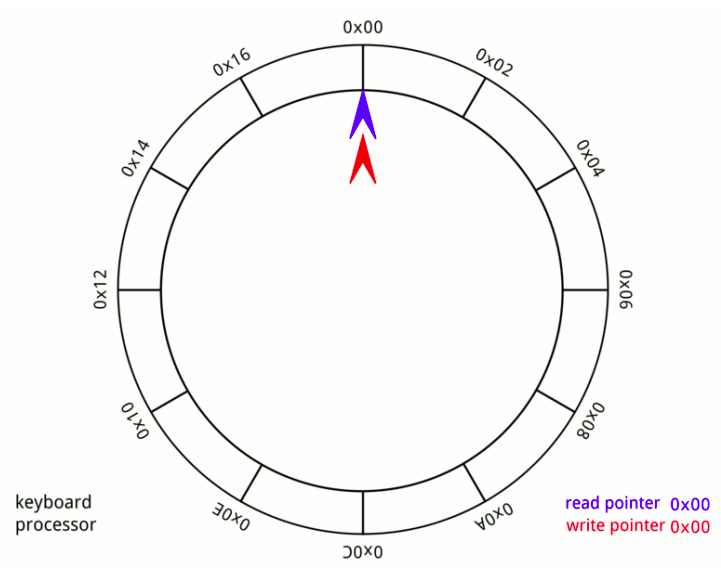
\includegraphics[align=c, width=0.50\textwidth]{coda-es-1.png}}
    \subfloat[Seconda scrittura]{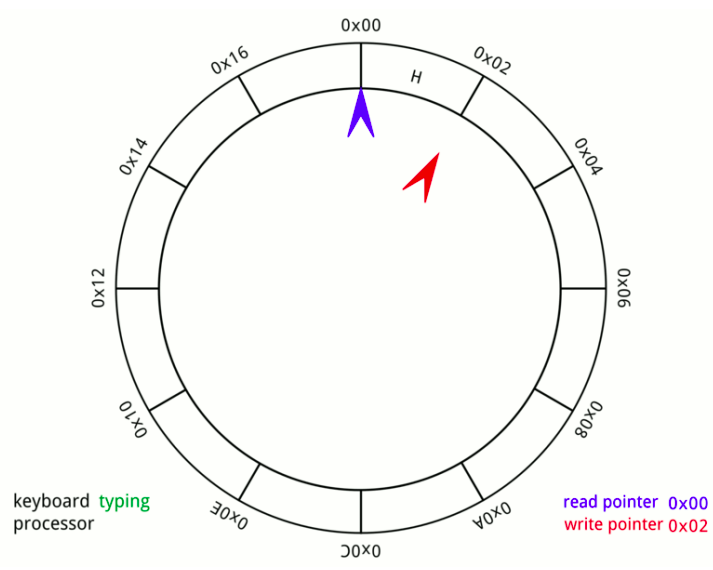
\includegraphics[align=c, width=0.50\textwidth]{coda-es-2.png}}\\
    \subfloat[Prima lettura]{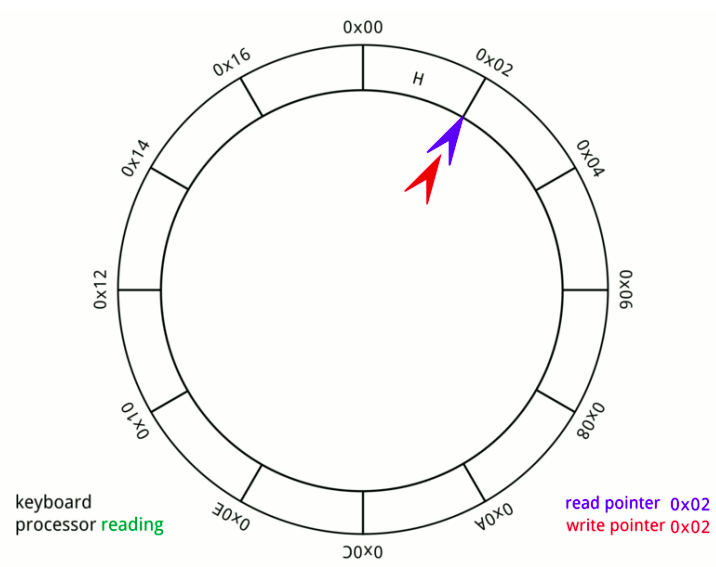
\includegraphics[align=c, width=0.50\textwidth]{coda-es-3.png}}
    \subfloat[Seconda lettura]{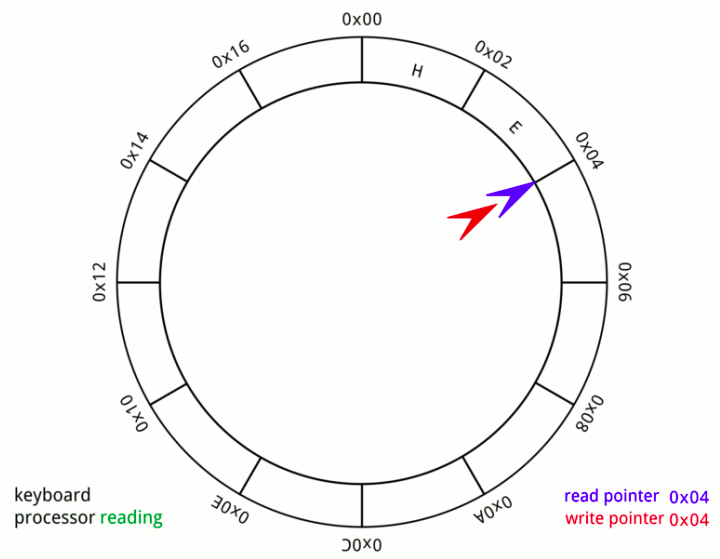
\includegraphics[align=c, width=0.50\textwidth]{coda-es-4.png}}\\
\end{figure}\newpage
\begin{figure}[ht]\ContinuedFloat
    \centering
    \subfloat[Ultima scrittura su cella libera]{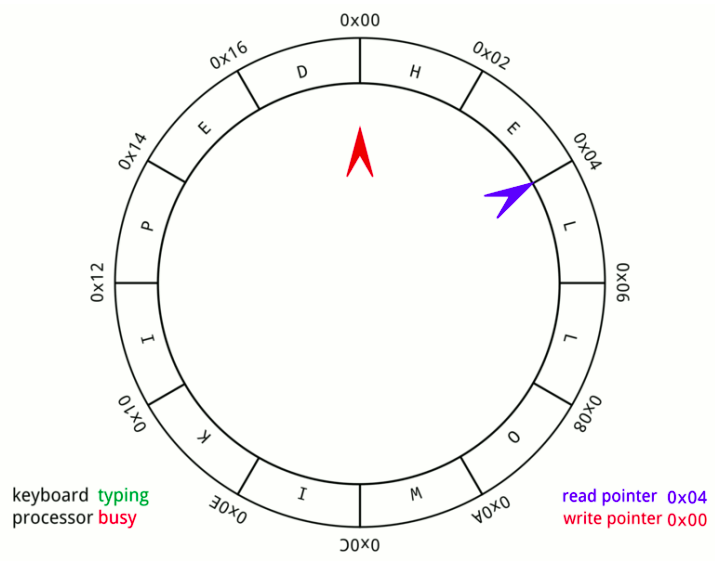
\includegraphics[align=c, width=0.50\textwidth]{coda-es-5.png}}
    \subfloat[Prima scrittura su cella già letta]{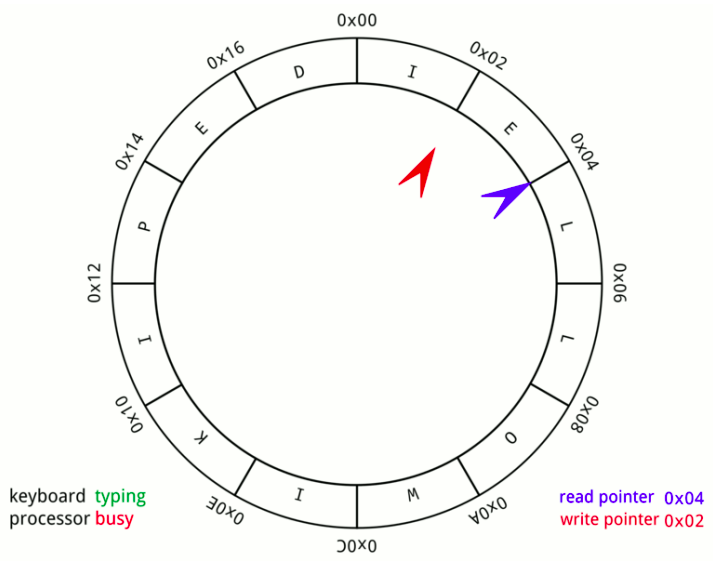
\includegraphics[align=c, width=0.50\textwidth]{coda-es-6.png}}\\
    \subfloat[Blocco delle scritture]{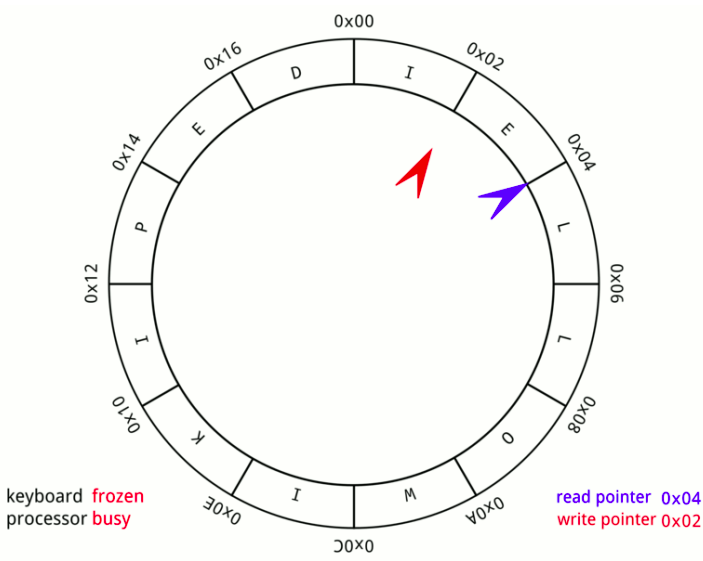
\includegraphics[align=c, width=0.50\textwidth]{coda-es-7.png}}
    \subfloat[Lettura di tutte le celle]{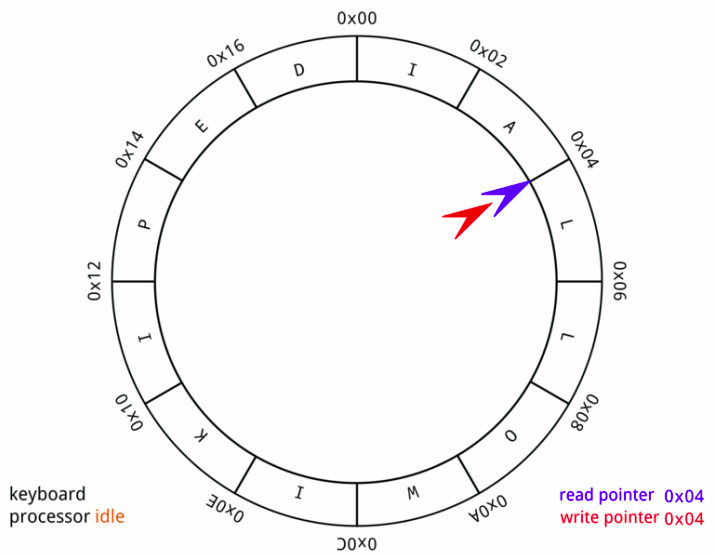
\includegraphics[align=c, width=0.50\textwidth]{coda-es-8.png}}
    \caption{Esempio di esecuzione di una \emph{coda} implementata come \emph{vettore circolare}}
\end{figure}\noindent
Nelle immagini di cui sopra si vede molto bene come, dopo ogni operazione di lettura
e scrittura, i rispettivi puntatori avanzino fino alla cella successiva.
Fino a quando ci sono celle libere i due puntatori avanzano in modo indipendente,
ma quando queste finiscono, le successive scritture vanno a sovrascrivere i
valori precedentemente inseriti e che sono stati già letti.

Una volta che il \emph{write pointer} si trova sulla cella che precede quella
indicata dal \emph{read pointer}, la \emph{coda} è piena e quindi non è possibile
inserire nuovi elementi fino a quando non ne vengono letti alcuni. Quando invece
il \emph{read pointer} va a sovrapporsi al \emph{write pointer} significa che la
\emph{coda} è stata svuotata e di conseguenza vengono bloccate le letture.

\newpage
\begin{code}{Coda basata su vettore circolare}
    \begin{minipage}[t]{0.48\textwidth}
        \bc{ITEM}[] V\hfill\com{Elementi}
        \bc{int} cur\_dim\hfill\com{Dimensione attuale}
        \bc{int} head\hfill\com{Testa della \emph{coda}}
        \bc{int} max\_dim\hfill\com{Dimensione massima}

        \ind\bc{QUEUE} Queue(\bc{int} dim)\\
            \bc{QUEUE} t = new \bc{QUEUE}\\
            t.V = new \bc{int}[dim]\\
            t.max\_dim = dim\\
            t.head = 0\\
            t.cur\_dim = 0\\
            return t\\

        \ind\bc{ITEM} top()\\
            precondition:(cur\_dim > 0)\\
            return V[head]\\
    \end{minipage}
    \hfill
    \begin{minipage}[t]{0.48\textwidth}
        \ind\bc{boolean} isEmpty()\\
            return (cur\_dim == 0)\\

        \ind\bc{ITEM} dequeue()\\
            precondition:(cur\_dim > 0)\\
            \bc{ITEM} t = V[head]\\
            head = (head + 1) mod max\_dim\\
            cur\_dim = cur\_dim - 1\\
            return t\\

        \ind enqueue(\bc{ITEM} v)\\
            precondition:(cur\_dim < max\_dim)\\
            V[(head + cur\_dim) mod max\_dim] = v\\
            cur\_dim = cur\_dim + 1
    \end{minipage}
\end{code}
\begin{note}
    In una \emph{coda} implementata come \emph{lista} non è necessario specificare
    una dimensione massima.
\end{note}